\documentclass[11pt]{article}

\usepackage[spanish]{babel}
\usepackage[utf8]{inputenc}
\usepackage[bookmarks=true, bookmarksnumbered=true, bookmarksopen=true, urlcolor=blue]{hyperref}
\usepackage{xcolor, multicol, multirow, longtable, graphicx}
\usepackage{amsmath, amssymb, amsthm}
\usepackage{tikz}
\usetikzlibrary{babel, cd}

\usepackage{pgfplots}
\pgfplotsset{
	colormap={ice}{HTML(0)=(3447d4); HTML(1)=(4188ea); HTML(2)=(80dcff); HTML(3)=(a4f8ff); HTML(4)=(d2feff)}
}

% Colores extra para el documento
\definecolor{newblue}{HTML}{4b80b7}
\definecolor{newgreen}{HTML}{69be28}
\definecolor{newred}{HTML}{ce1a1a}

% Comandos definidos en los ejemplos
\definecolor{sample}{HTML}{00c89c}
\DeclareMathOperator{\mcd}{mcd}
\DeclareMathOperator*{\dom}{dom}
\newtheorem{thm}{Teorema}
\newtheorem{mydef}{Definición}[section]
\newtheorem{cor}[mydef]{Corolario}
\newtheorem*{note}{Observación}

\usepackage{textcomp}
\newenvironment{demo}[1][$\bullet$]{#1 {\scshape Demostración:} }{\par\noindent}

% Comandos para escribir código entre párrafos
\usepackage{listings}
\lstset{
	language        = {[LaTeX]TeX},
	backgroundcolor = \color{black!17},
	basicstyle      = \small\ttfamily,
	breaklines      = true,
	commentstyle    = \itshape\color{gray},
	frame           = tb,
	moredelim       = **[is][\itshape]{¬}{¬},
	morekeywords    = {@book, \maketitle, \chapter, \part, \subsection, \subsubsection, \color, \definecolor,
	                  \textcolor, \colorbox},
	keywordstyle    = \color{newblue},
	showspaces      = false,
	tabsize         = 4,
	classoffset     = 1,
	morekeywords    = {\nexists, \varnothing, \complement, \beth, \gimel, \square, \blacksquare, \dfrac, \tfrac, \binom,
			  \includegraphics, \DeclareMathOperator, \addbibresource, \printbibliography, \multirow, \eqref,
			  \operatorname, \text, \addplot, \addlegendentry},
	keywordstyle    = \color{violet},
	classoffset     = 0,
	literate        = {á}{{\'a}}1 {é}{{\'e}}1 {í}{{\'i}}1 {ó}{{\'o}}1 {ú}{{\'u}}1 {ñ}{{\~n}}1
	                  {Á}{{\'A}}1 {É}{{\'E}}1 {Í}{{\'I}}1 {Ó}{{\'O}}1 {Ú}{{\'U}}1 {Ñ}{{\~N}}1,
}

\title{Introducción breve a \LaTeX}
\author{
	José Cuevas Barrientos\\
	\small\color{teal}\url{https://github.com/JoseCuevasBtos/apuntes-tex}
}
\date\today

\begin{document}

\maketitle
\tableofcontents

\section{Introducción}
Este texto pretende ser introductorio y en general sólo abarca cosas que creo que un lector cualquiera podría necesitar a la hora de usar \LaTeX{}. Por su naturaleza, sólo se roza la superficie de lo que es posible en este lenguaje, si lo que busca es una documentación más detallada revise el párrafo de \textbf{Más allá...} al final de la sección~\S\ref{sec:setup}.

Respecto de la instalación de \LaTeX{}, para ello están los compiladores de Mik\TeX{} en Windows, Mac\TeX{} en Mac OS y \TeX{}Live en Linux. Los editores recomendados son \TeX{}Maker y \href{https://www.overleaf.com/}{\sffamily\color{newgreen}overleaf} (en línea). Para usuarios de Vim, recomiendo usar el plugin \href{https://github.com/lervag/vimtex}{\ttfamily vimtex}.

\section{Haciendo un documento básico desde cero}
En primera vamos a ver la estructura y características generales de \LaTeX{}. A diferencia de MS Word, \LaTeX{} no es un generador WYSIWYG\footnote{en. \textit{what you see is what you get}; lo que ves es lo que obtienes.}, sino que se escribe mediante texto en un archivo de texto y un lenguaje de marcado. No os confundas, \LaTeX{} \textbf{no} es un lenguaje de programación, y no se parece a uno, sino que es como escribir texto común con comandos entre medio.

\subsection{``Hola mundo''}
Los comandos suelen tener esta estructura \lstinline|\comando{¬opciones¬}| donde la información obligatoria para el comando suele ir entre llaves \texttt{\{\}} a los que llamaremos \textit{campos obligatorios}, mientras que la información opcional suele ir entre corchetes \texttt{[]}. Todo documento comienza así:
\begin{lstlisting}
\documentclass[¬opciones¬]{¬tipo de documento¬}
\end{lstlisting}
Por el momento en las opciones incluiremos el tamaño normal de letra que es 10, 11 o 12pt y el tipo de documento será \texttt{article} o \texttt{book} según lo que se desee escribir.

Luego viene un comando de la forma:
\begin{lstlisting}
\begin{document}
Hola mundo.
\end{document}
\end{lstlisting}
Varios comandos tendran la misma estructura, a estos les llamaremos \textit{entornos} y a la parte de \texttt{document} su ``tag''. El entorno \texttt{document} señala todo lo perteciente al contenido del archivo. Todo lo que esté fuera de este entorno (en particular antes de él) le diremos la \textit{cabecera} del documento. Debería compilar este archivo básico para corroborar que su instalación de \LaTeX{} ha sido exitosa. Varios programas (como TeXMaker) tienen compiladores incluidos, pero si se interesa en hacerlo por la terminal puede ver el apéndice.

\textbf{Paquetes.} Igual que los lenguajes de programación permiten añadir módulos para añadir funciones (como \texttt{<stdio.h>} en \texttt{C}, o \texttt{numpy} en \texttt{Python}), \LaTeX{} ocupa paquetes que se incluyen en la cabecera, de momento añadiremos dos:
\begin{lstlisting}
\usepackage[spanish]{babel}
\usepackage[utf8]{inputenc}
\end{lstlisting}
El primero le indica a \LaTeX{} que estamos escribiendo en español, para traducir texto del documento como escribir ``Capítulo'' en lugar de ``Chapter''. El segundo le dice a \LaTeX{} que lea las tildes y otros caracteres especiales (e.g. á, ñ, ç, etc.) sin problema.

\textbf{Título.} (Casi) todo documento tiene cosas como título, autor y fecha, para incluirlos en \LaTeX{} debe ocupar correspondientemente los siguientes comandos en la cabecera:
\begin{lstlisting}
\title{Mí título interesante}
\author{Yo}
\date{\today}
\end{lstlisting}
Nótese que en la fecha utilice el comando \lstinline|\today|, este lee la fecha del día en el computador y el paquete de \texttt{babel} lo traduce al español, pero puede ocupar cualquier otra que se le antoje. Dentro del documento y antes del resto del texto escriba este comando para generar el título estándar de \LaTeX{}:
\begin{lstlisting}
\maketitle
\end{lstlisting}

\textbf{Secciones.} Todo texto suele dividirse en secciones. \LaTeX{} también, y además las enumera automáticamente. En un artículo la mayor división es una sección, luego una subsección y luego una sub-subsección:
\begin{lstlisting}
\section{Esta es mi sección}
\subsection{Esta mi subsección}
\subsubsection{Esta mi sub-subsección}
\end{lstlisting}
Un libro también admite todos los comandos anteriores, pero la mayor distinción es un capítulo \lstinline|\chapter{...}| y se pueden agrupar los capítulos en partes \lstinline|\part{...}|, donde las últimas se enumeran con números romanos; pero a diferencia de los capítulos no son obligatorios.

\textbf{Cortes de línea.} Cuando hay un salto entre punto aparte y el otro párrafo eso se dice un \textit{corte de línea}, lo que uno está acostumbrado a hacer con la tecla \texttt{Enter} de vuestros teclados. No obstante en el código de \LaTeX{} puede notar que no genera efecto alguno, esto se debe a que en los lenguajes de marcado se da esta precaución para evitar líneas excesivamente largas en el código.
Para hacer este corte hay varias formas: \lstinline|\\| suele ser el más común, y no genera sangría en la línea contigua. Para hacer un corte con sangría puede usar dos veces \texttt{Enter} en el código. Un efecto similar es el de usar \lstinline|\par|. La sangría se puede añadir con \lstinline|\indent| y quitar con \lstinline|\noindent| de ser necesario. Por último, si necesita forzar un corte de línea, para evitar la sobrecarga de caractéres por ejemplo, puede usar \lstinline|\break|.
\begin{multicols}{2}
	\begin{lstlisting}
Texto de ejemplo.\break
Texto de ejemplo.\\
Texto de ejemplo.\par
Texto de ejemplo.
	\end{lstlisting}
	Texto de ejemplo.\break
	Texto de ejemplo.\\
	Texto de ejemplo.\par
	Texto de ejemplo.
\end{multicols}

\textbf{Caracteres especiales.} Sabemos que los comandos se inician con \lstinline|\|, por ende, ¿cómo se escribe dicho caracter de ser necesario en \LaTeX{}? Esta clase de caracteres se dicen \textit{especiales} pues cumplen una función por si solos y se pueden escribir así:
\begin{figure}[!h]
	\centering
	\begin{tabular}{ll|ll}
		\hline \hline
		\lstinline|$\backslash$| & $\backslash$ & \lstinline|\_|           & \_ \\
		\lstinline|\%|           & \%           & \lstinline|\#|           & \# \\
		\lstinline|\$|           & \$           & \lstinline|\&|           & \& \\
		\lstinline|\{\}|         & \{\} \\
		\hline \hline
	\end{tabular}
\end{figure}

Además debe tener en consideración que las comillas en \LaTeX{} son también distintas para escribir algo ``así'' se requiere \lstinline|``así''|. Donde las dos primeras son tildes graves y las últimas son apostrofes.

\subsection{Formato de texto}
\textbf{Estilos.} Uno suele cambiar el formato, e.g. a \textbf{negritas}, o \textit{cursivas}, para ello \LaTeX{} ocupa:
\begin{figure}[!h]
	\centering
	\begin{tabular}{lll}
		\hline \hline
		\lstinline|\textup{Derecho}|     & \lstinline|\upshape|  & \textup{Derecho}\\
		\lstinline|\textit{Cursivas}|    & \lstinline|\itshape|  & \textit{Cursivas}\\
		\lstinline|\textsl{Inclinado}|   & \lstinline|\slshape|  & \textsl{Inclinado}\\
		\lstinline|\textsc{Versallitas}| & \lstinline|\scshape|  & \textsc{Versallitas}\\
		\hline
		\lstinline|\textmd{Mediano}|     & \lstinline|\mdseries| & \textmd{Mediano}\\
		\lstinline|\textbf{Negritas}|    & \lstinline|\bfseries| & \textbf{Negritas}\\
		\hline
		\lstinline|\textrm{Romano}|      & \lstinline|\rmfamily| & \textrm{Romano}\\
		\lstinline|\textsf{Sans-serif}|  & \lstinline|\sffamily| & \textsf{Sans-serif}\\
		\lstinline|\texttt{Máquina}|     & \lstinline|\ttfamily| & \texttt{Máquina}\\
		\hline \hline
	\end{tabular}
\end{figure}

El segundo tipo de comando es lo que se dice un \textit{modificador}, al usarlo modifica todo el entorno\footnote{En realidad modifica el entorno restante, ya que el contenido dentro del mismo entorno que viene ántes del modificador no se ve afectado.}, e.g., \lstinline|{\scshape Texto de Ejemplo}| {\scshape Texto de Ejemplo}.

\textbf{Tamaños.} Para los tamaños de letra puedes usar un modificador o un entorno, ambos ocupan el mismo tag:
\begin{center}
	{\tiny tiny}
	{\scriptsize scriptsize}
	{\footnotesize footnotesize}
	{\small small}
	{\normalsize normalsize}\\
	{\large large}
	{\Large Large}
	{\LARGE LARGE}
	{\huge huge}
	{\Huge Huge}
\end{center}
Cambiar el tamaño de letra por defecto (de 10 a 12pt por ejemplo) afecta también los otros tamaños de letra.

\textbf{Alineación.} \LaTeX{} permite de dos formas el cambio de alineación de texto:
\begin{figure}[!h]
	\centering
	\begin{tabular}{lll}
		\hline \hline
		Alineación & Entorno             & Modificador \\
		\hline
		Izquierda  & \texttt{flushleft}  & \lstinline|\raggedright| \\
		Derecha    & \texttt{flushright} & \lstinline|\raggedleft| \\
		Centro     & \texttt{center}     & \lstinline|\centering| \\
		\hline \hline
	\end{tabular}
\end{figure}

\textbf{Colores.} Para admitir colores extra se debe importar el siguiente paquete en la cabecera:
\begin{lstlisting}
\usepackage{xcolor}
\end{lstlisting}
Para usarlo puedes escribir: \lstinline|{\color{red} texto en rojo}| {\color{red} texto en rojo} o\break
\lstinline|\textcolor{blue}{texto en azúl}| \textcolor{blue}{texto en azúl}. Los nombres de colores por defecto son:
\begin{multicols}{5}
	\noindent\ttfamily
	\colorbox{black}{\color{white} black}\\
	\colorbox{blue}{blue}\\
	\colorbox{brown}{brown}\\
	\colorbox{cyan}{cyan}\\
	\colorbox{darkgray}{\color{white} darkgray}\\
	\colorbox{gray}{gray}\\
	\colorbox{green}{green}\\
	\colorbox{lightgray}{lightgray}\\
	\colorbox{lime}{lime}\\
	\colorbox{magenta}{magenta}\\
	\colorbox{olive}{olive}\\
	\colorbox{orange}{orange}\\
	\colorbox{pink}{pink}\\
	\colorbox{purple}{\color{white} purple}\\
	\colorbox{red}{red}\\
	\colorbox{teal}{teal}\\
	\colorbox{violet}{\color{white} violet}\\
	\colorbox{white}{white}\\
	\colorbox{yellow}{yellow}
\end{multicols}
Para poner colores en el fondo se utiliza \lstinline|\colorbox{cyan}{Así}| \colorbox{cyan}{Así}. Además puedes utilizar un porcentaje de un color, por ejemplo, si sólo queremos usar el 50\% de negro podemos escribir \lstinline|\colorbox{black!50}{esto}| \colorbox{black!50}{esto}, y si queremos usar 50\% azúl y el resto rojo \lstinline|\colorbox{blue!50!red}{haga esto}| \colorbox{blue!50!red}{haga esto}.

Por sobre eso, usted puede definir nuevos colores en la cabecera:
\begin{lstlisting}
\definecolor{ejemplo}{HTML}{00c89c}
\end{lstlisting}
Donde lo de \texttt{HTML} indica que la forma de definir colores es mediante el llamado código hexadecimal o \texttt{hex} para acortar. Este suele ser el método más común de definir colores, en línea lo reconocerá pues ocupan el prefijo `\texttt{\#}', e.g., \texttt{\color{sample}\#00c89c}.

\textbf{Varias columnas.} Si usted quisiera, de forma global, tener un documento escrito en dos columnas, sólo basta agregar la opción \texttt{twocolumn} en \lstinline|\documentclass|. No obstante, si desea hacerlo localmente, esto es, en una sola parte del documento, debe importar el paquete:
\begin{lstlisting}
\usepackage{multicol}
\end{lstlisting}
y luego usar el entorno \texttt{multicols} seguido del número de columnas:
\begin{lstlisting}
\begin{multicols}{2}
	Muchos años después, frente al pelotón de fusilamiento, el coronel Aureliano Buendía...
\end{multicols}
\end{lstlisting}
\begin{multicols}{2}
	Muchos años después, frente al pelotón de fusilamiento, el coronel Aureliano Buendía había de recordar aquella tarde remota en que su padre lo llevó a conocer el hielo. Macondo era entonces una aldea de veinte casas de barro y cañabrava construidas a la orilla de un río de aguas diáfanas que se precipitaban por un lecho de piedras pulidas, blancas y enormes como huevos prehistóricos.
\end{multicols}

\subsection{Notas, listas, figuras y tablas}
\textbf{Notas.} \LaTeX{} admite dos tipos comúnes de notas: al pie de la página y al margen de ella. La primera se especifica con el comando \lstinline|\footnote{Esta es una nota al pie de página.}|\footnote{Esta es una nota al pie de página.} mientras que las notas de margen se hacen con \lstinline|\marginpar{Y ésta, una nota al margen.}|\marginpar{Y ésta, una nota al margen.}. Para revertir el lugar se puede usar \lstinline|\reversemarginpar{...}|.

Para más información y mejor manejo de las notas al margen se recomienda revisar el paquete \texttt{marginnote}.

\textbf{Listas.} Se dividen en tres: numeradas, no numeradas y descripciones (similar a un glosario o diccionario). Todas se definen por un entorno y sus elementos se diferencian por el comando \lstinline|\item|. Para una lista enumerada el entorno utiliza el tag \texttt{enumerate}, las no numeradas el tag \texttt{itemize} y las descripciones \texttt{description}. En las descripciones, la palabra (o frase) de título se denota en el campo opcional de \lstinline|\item[¬Aquí...¬]|. Por ejemplo:
\begin{lstlisting}[basicstyle=\footnotesize\ttfamily]
\begin{enumerate}
	\item Naranjas.
	\item Manzanas:
		\begin{itemize}
			\item Rojas.
			\item Verdes.
			\item Amarillas.
		\end{itemize}
	\item Bananas.
\end{enumerate}
\begin{description}
	\item[Fruta] Fruto comestible de ciertas plantas cultivadas; e.g., la pera, la guinda, la fresa, etc.
	\item[Verdura] Hortaliza, especialmente la de hojas verdes.
\end{description}
\end{lstlisting}
\begin{enumerate}
	\item Naranjas.
	\item Manzanas:
		\begin{itemize}
			\item Rojas.
			\item Verdes.
			\item Amarillas.
		\end{itemize}
	\item Bananas.
\end{enumerate}
\begin{description}
	\item[Fruta] Fruto comestible de ciertas plantas cultivadas; e.g., la pera, la guinda, la fresa, etc.
	\item[Verdura] Hortaliza, especialmente la de hojas verdes.
\end{description}

\textbf{Figuras y tablas.} Por defecto, \LaTeX{} no permite importar imágenes al documento por lo que se requiere importar el paquete:
\begin{lstlisting}
\usepackage{graphicx}
\end{lstlisting}
Luego para importar la figura (asumiendo que la imágen está en la misma carpeta que el archivo) se utiliza el siguiente comando:
\begin{lstlisting}
\includegraphics[¬opciones¬]{imagen.jpg}
\end{lstlisting}
En las opciones usualmente van especificaciones sobre el tamaño, verá que sin ella la figura se importa al máximo tamaño para el cual no pierde detalle, para importarlo digamos a la mitad de su tamaño real puede usar \texttt{scale=.5}, pero usualmente es mejor especificar directamente ya sea el largo (\texttt{width}) o el alto (\texttt{height}) del archivo que debe hacerse en \texttt{cm}, \texttt{mm} o \texttt{in} (pulgadas). También podemos decirle que sea tan larga como el tamaño del texto usando \lstinline|width=\textwidth|.

Para que la imagen este apartada del texto se incluye todo dentro de un entorno \texttt{figure} cuyo único propósito es ese de decirle a \LaTeX{} que trate la imagen individualmente. Dentro de él se recomienda centrar el texto (o en este caso el contenido) y al final del entorno se recomienda añadir alguna forma de corte de línea para mejorar el formato.

\textbf{Posicionamiento.} Para saber donde ubicar la imagen, \LaTeX{} utiliza los siguientes símbolos para abreviar:
\begin{figure}[!h]
	\centering
	\begin{tabular}{lp{8cm}}
		\hline \hline
		\texttt{h} & Aproximadamente en el lugar donde se ubica en el código. \\
		\texttt{t} & En el tope de la página siguiente. \\
		\texttt{b} & En el fondo de la página actual. \\
		\texttt{p} & En la siguiente página, destinada exclusivamente para figuras. \\
		\texttt{!} & Fuerza la posición indicada. \\
		\hline \hline
	\end{tabular}
\end{figure}

\textbf{Descripciones.} Además las imágenes poseen descripciones cortas, estas pueden agregarse en \LaTeX{} dentro de un entorno \texttt{figure} con el comando \lstinline|\caption{Mi descripción.}|, veamos un ejemplo donde se utiliza todo lo anterior:
\begin{lstlisting}
\begin{figure}[!h]
	\centering
	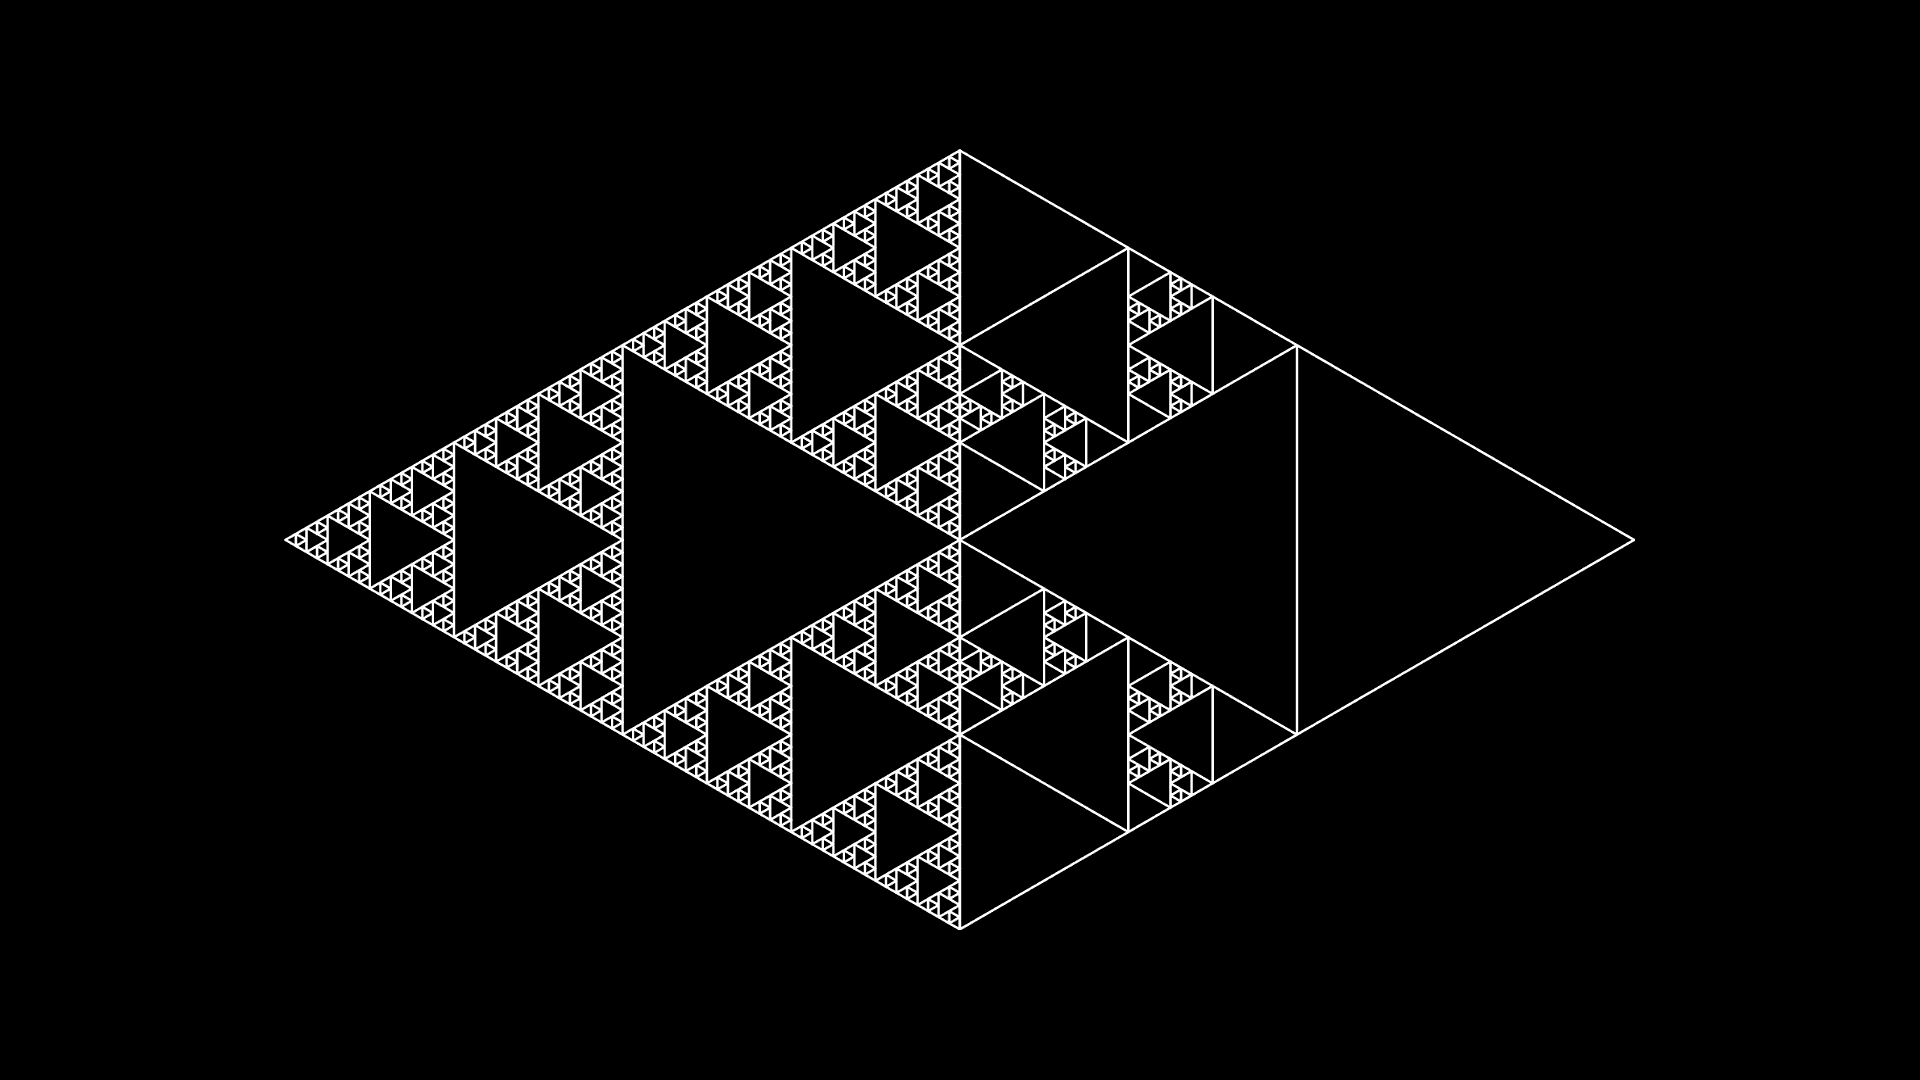
\includegraphics[width=10cm]{fractal.png}
	\caption{Un fractal}
\end{figure}
\end{lstlisting}
\begin{figure}[!h]
	\centering
	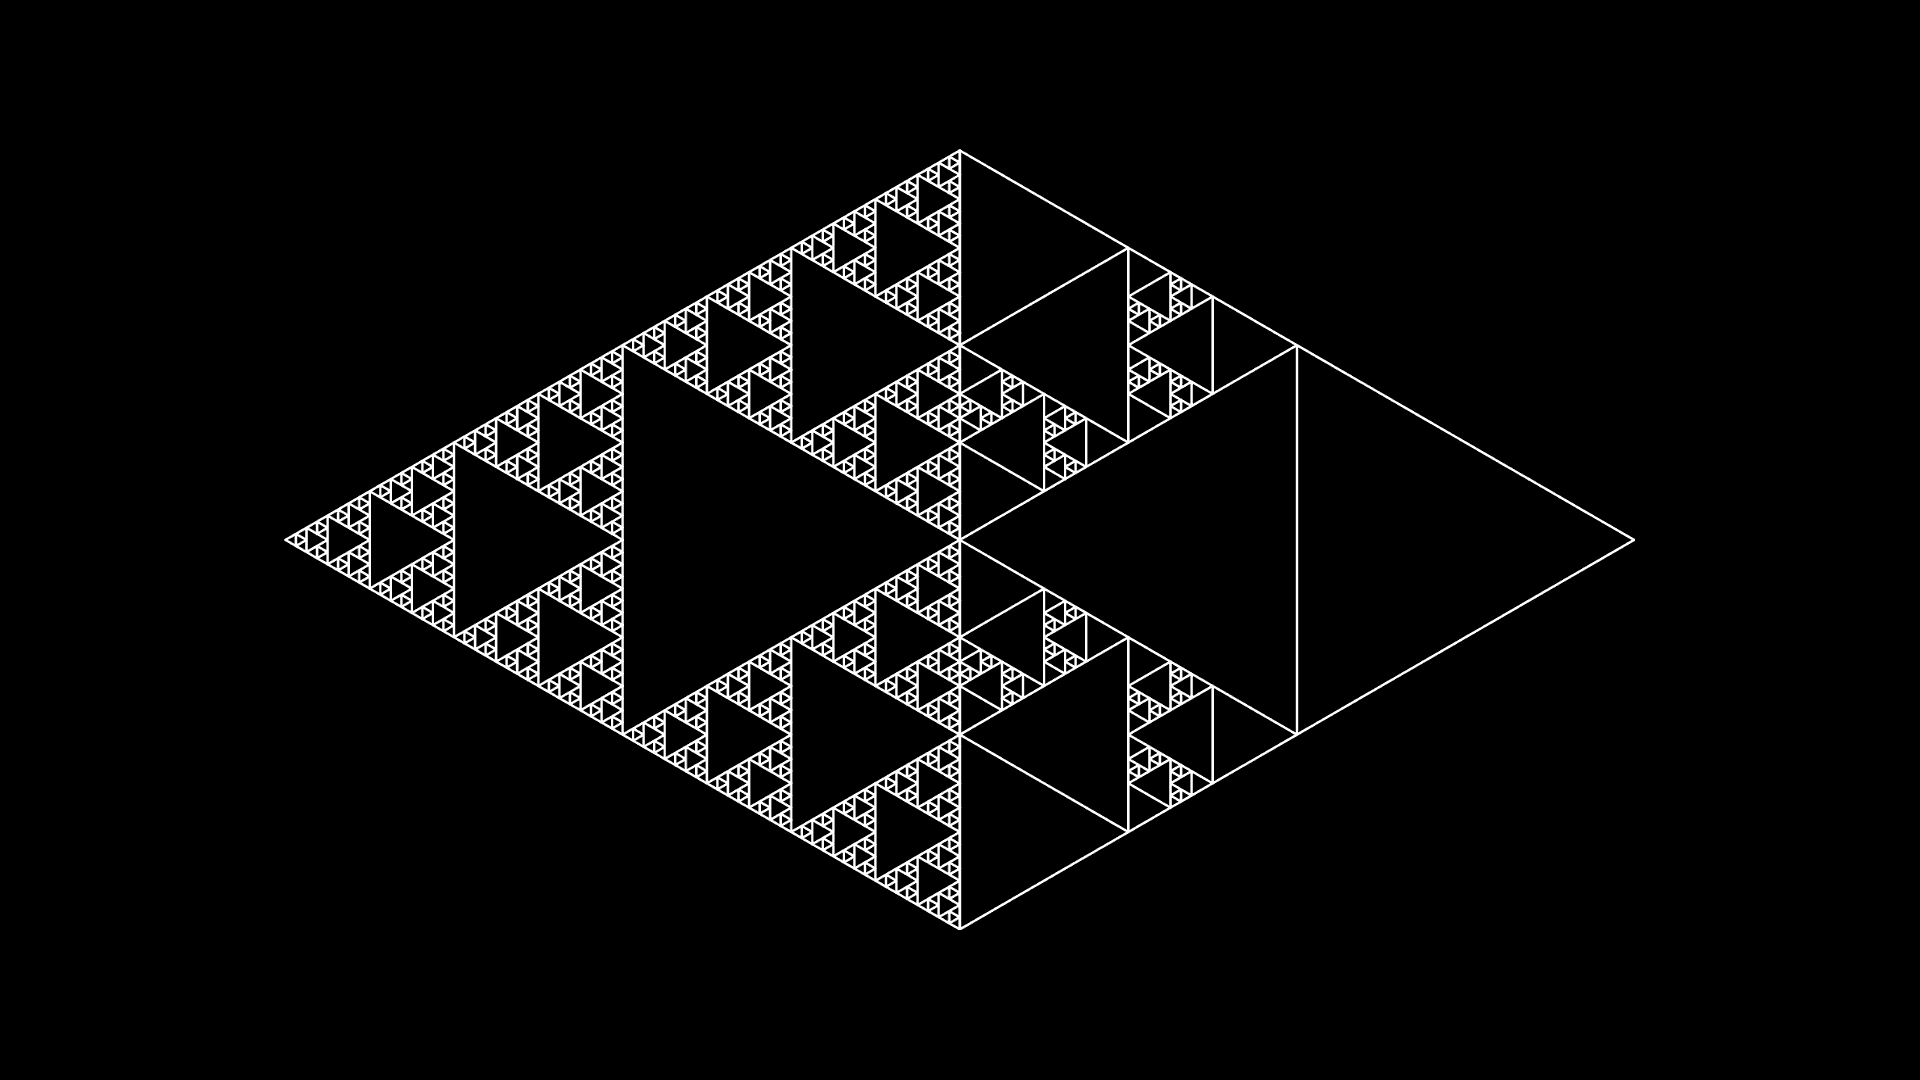
\includegraphics[width=10cm]{fractal.png}
	\caption{Un fractal}
\end{figure}

\textbf{Tablas.} Las tablas se definen así:
\begin{lstlisting}
\begin{tabular}{¬formato¬}
	...
\end{tabular}
\end{lstlisting}
Donde el \textit{formato} se define por lo siguiente:
\begin{table}[!h]
	\centering
	\begin{tabular}{lp{8cm}}
		\hline \hline
		\lstinline|l|	     & Celdas hacia la izquierda. \\
		\lstinline|c|	     & Celdas centradas. \\
		\lstinline|r|	     & Celdas hacia la derecha. \\
		\lstinline|p{¬longitud¬}| & Párrafo de cierta longitud. \\
		\lstinline|m{¬longitud¬}| & Como \texttt{p}, pero centrado verticalmente\textsuperscript{\dag}. \\
		\lstinline|b{¬longitud¬}| & Como \texttt{p}, pero verticalmente al fondo\textsuperscript{\dag}. \\
		\hline \hline
	\end{tabular}
\end{table}

Los marcados por \dag{} requieren del paquete \texttt{array}. Las celdas en una columna se separan por el símbolo \texttt{\&} y las columnas se separan por un corte de línea. Además \lstinline|\hline| genera una línea horizontal lo que puede ser útil. Tal como uno pone las figuras en un entorno \texttt{figure}, existe el entorno \texttt{table} para tablas que sirve para posicionar y añadir descripciones; funciona exactamente igual.
\begin{lstlisting}
\begin{table}[!h]
	\centering
	\begin{tabular}{|lcc|}
		\hline
		País & Contagios totales & Fallecidos totales \\
		\hline \hline
		Argentina & 201,919 & 3,667 \\
		Chile     & 361,493 & 9,707 \\
		Colombia  & 317,651 & 10,650 \\
		Peru      & 428,850 & 19,614 \\
		\hline
	\end{tabular}
	\caption{Estado Covid-19 (3 de agosto de 2020).}
\end{table}
\end{lstlisting}
\begin{table}[!h]
	\centering
	\begin{tabular}{|lcc|}
		\hline
		País & Contagios totales & Fallecidos totales \\
		\hline \hline
		Argentina & 201,919 & 3,667 \\
		Chile     & 361,493 & 9,707 \\
		Colombia  & 317,651 & 10,650 \\
		Peru      & 428,850 & 19,614 \\
		\hline
	\end{tabular}
	\caption{Estado Covid-19 (3 de agosto de 2020).}
\end{table}

Se puede agrupar un formato y repetir $n$ veces con la abreviación \lstinline|*{¬n¬}{¬formato¬}|. En el ejemplo anterior podríamos reemplazar la \lstinline|cc| por \lstinline|*{2}{c}|. Una celda puede usar el tamaño de varias dentro de la misma fila usando el comando \lstinline|\multicolumn{¬num¬}{¬form¬}{¬contenido¬}| donde \textit{num} es el número de columnas que abarca, y \textit{form} el formato de ella, e.g:
\begin{lstlisting}[basicstyle=\footnotesize\ttfamily]
\begin{table}[!h]
	\centering
	\begin{tabular}{|l|cc|}
		\hline
		País & Contagios totales & Nuevos contagios \\
		\hline \hline
		\multicolumn{3}{|c|}{\sffamily América} \\
		\hline
		EEUU        & 4,851,407 & +38,379 \\
		Brasil      & 2,736,298 & +2,621  \\
		\hline
		\multicolumn{3}{|c|}{\sffamily Europa} \\
		\hline
		Reino Unido & 305,623   & +928    \\
		Italia      & 248,229   & +159    \\
		\hline
	\end{tabular}
\end{table}
\end{lstlisting}
\begin{table}[!h]
	\centering
	\begin{tabular}{|l|cc|}
		\hline
		País & Contagios totales & Nuevos contagios \\
		\hline \hline
		\multicolumn{3}{|c|}{\sffamily América} \\
		\hline
		EEUU        & 4,851,407 & +38,379 \\
		Brasil      & 2,736,298 & +2,621  \\
		\hline
		\multicolumn{3}{|c|}{\sffamily Europa} \\
		\hline
		Reino Unido & 305,623   & +928    \\
		Italia      & 248,229   & +159    \\
		\hline
	\end{tabular}
\end{table}

Con el paquete \texttt{multirow} puedes combinar filas también mediante el comando \lstinline|\multirow{¬num¬}{¬longitud¬}{¬contenido¬}| (puedes usar \texttt{*} en el lugar de la longitud para ocupar todo lo disponible). Y puedes hacer líneas horizontales parciales desde el inicio de la $i$-ésima celda hasta el final de la $j$-ésima celda con \lstinline|\cline{¬i-j¬}|, e.g.:
\begin{lstlisting}[basicstyle=\footnotesize\ttfamily]
\begin{table}[!h]
	\centering
	\begin{tabular}{|l|lcc|}
		\cline{2-4}
		\multicolumn{1}{c|}{}    & País   & Contagios totales & Nuevos contagios \\
		\hline
		\multirow{2}{*}{América} & EEUU   & 4,851,407         & +38,379 \\
		\cline{2-4}
		{}                       & Brasil & 2,736,298         & +2,621  \\
		\hline
	\end{tabular}
\end{table}
\end{lstlisting}
\begin{table}[!h]
	\centering
	\begin{tabular}{|l|lcc|}
		\cline{2-4}
		\multicolumn{1}{c|}{}    & País   & Contagios totales & Nuevos contagios \\
		\hline
		\multirow{2}{*}{América} & EEUU   & 4,851,407         & +38,379 \\
		\cline{2-4}
		{}                       & Brasil & 2,736,298         & +2,621  \\
		\hline
	\end{tabular}
\end{table}
\textbf{Tablas entre páginas.} Por defecto \LaTeX{} no rompe una tabla entre páginas, sin importar cuan larga sea, para poder usar un \textit{tabla larga} se debe importar el paquete \texttt{longtable} que provee el entorno homónimo que funciona exactamente igual que \texttt{tabular}.

\subsection{Bibliografías, referencias cruzadas e índices}
\label{sec:crossref}
\LaTeX{} es bastante popular por su forma de tratar bibliografías, por lo cual vamos a enseñar como: En primer lugar, todas las referencias bibliográficas se guardan en otro archivo externo de extensión \texttt{.bib}. Para incluir una bibliografía debemos añadir el siguiente comando:
\begin{lstlisting}
\usepackage[backend=biber]{biblatex}
\addbibresource{¬mis-referencias¬.bib}
\end{lstlisting}
Y para compilarlo hay que compilar el documento una primera vez, luego compilar la bibliografía con \textit{biber} y luego una segunda vez. Esto se debe a que la primera vez le dice a \LaTeX{} que referencias crear, luego el compilador las crea con su respectivo formato y la última las incluye.

Las referencias se pueden buscar facilmente en páginas como \url{https://scholar.google.com/} y luego seleccionando obtener el formato en Bib\TeX{} o similar. En general toda referencia suele verse así:
\begin{lstlisting}
@book{gauss1966disquisitiones,
	title={Disquisitiones arithmeticae},
	author={Gauss, Carl Friedrich},
	volume={157},
	year={1966},
	publisher={Yale University Press}
}
\end{lstlisting}
Donde es bastante claro como funciona, la palabra \texttt{book} indica que la referencia es un libro, \texttt{gauss1966disquisitiones} es lo que le decimos una \textit{etiqueta}, i.e., una cadena de signos sin espacios que se utiliza para citar dentro del documento, luego el resto es claro. Lo único importante a saber es que en el campo del autor se recomienda anotar apellido, luego coma, luego nombre; y si hay más de uno separarlos por la palabra \texttt{and}, si hay muchos y se quiere utilizar algo para decir ``y otros'' (et al. en latín) se utiliza un \texttt{others} (Albert Einstein et al. sería \texttt{Einstein, Albert and others} para \LaTeX{}).

Usualmente se utiliza un solo archivo general para tener todas las referencias allí, luego, utilizando el ejemplo anterior, uno citaría un documento así:
\begin{lstlisting}
\cite{gauss1966disquisitiones}
\end{lstlisting}
Si se quiere que la cita este al pie de página uno ocupa \lstinline|\footcite{...}| y puedes citar varios documentos juntos separando las etiquetas por comas. Entre las referencias sólo aparecerán los trabajos citados. Para incluir un trabajo sin citarlo en la bibliografía debemos usar el comando \lstinline|\nocite{...}| donde las mismas reglas se aplican.
Si se quiere incluir a todas las referencias puedes escribir \lstinline|\nocite{*}|. 
Para imprimir las bibliografías se ocupa este comando:
\begin{lstlisting}
\printbibliography
\end{lstlisting}

\textbf{Sub-bibliografías y palabras clave.} No obstante, un problema que puede surgir al tratar bibliografías es que toman un capítulo (o sección si de un artículo se trata) entero cuando se imprimen, y un formato interesante es el de ciertos libros que usan bibliografía para cada capítulo, lo que por el momento parece una tarea imposible. Un problema similar es si queremos incluir muchos artículos a la vez, pero no todos y sólo queremos incluir los de un cierto tema. Para ambos la solución implica introducir el mismo concepto: palabras clave.

Dentro de la definición de libros en Bib\TeX{} se añade la categoría \texttt{keywords} (sí, plural) donde especifica las palabras clave separadas por comas. Tomemos el ejemplo del libro de Gauss y supongamos que le añadimos \lstinline|keywords={arithmetic}| donde tenemos varias referencias marcadas sobre el tema de \texttt{arithmetic} luego este comando:
\begin{lstlisting}
\printbibliography[keyword={arithmetic}]
\end{lstlisting}
Imprimirá sólo dichos artículos. Para el problema de las sub-bibliografías añada la opción de \texttt{subbibintoc}. Y para cambiarle el nombre puede usar la opción, \lstinline|heading={¬mi título¬}|.

\textbf{Referencias cruzadas.} Una de las ventajas de \LaTeX{} es que como genera automáticamente la numeración para las secciones, figuras y ecuaciones, se pueden referenciar de forma bastante sencilla, junto a uno de esos entornos se agrega el comando \lstinline|\label{¬etiqueta¬}| y luego se llama con \lstinline|\ref{¬etiqueta¬}| (puede requerir una compilación doble para funcionar adecuadamente), e.g:
\begin{lstlisting}[basicstyle=\footnotesize\ttfamily]
\subsection{Bibliografías, referencias cruzadas e índices}
\label{sec:crossref}
---------------------------------------------------
...similar a lo dicho en la sección \ref{sec:crossref}.
\end{lstlisting}
...similar a lo dicho en la sección \ref{sec:crossref}.

La parte de \texttt{sec:} es una costumbre decorativa, así como se suele usar \texttt{eq:} como prefijo para las ecuaciones, \texttt{fig:} para las figuras, etc. No es necesaria pero puede servir para ordenarse en el código fuente.

\textbf{Tablas de contenidos.} La tabla de contenidos no puede ser más fácil de implementar, sólo basta con el comando:
\begin{lstlisting}
\tableofcontents
\end{lstlisting}
Además se pueden usar \lstinline|\listoftables| y \lstinline|\listoffigures| para imprimir índices de las tablas y las figuras del documento (sólo ocupa las entradas  con descripciones, puedes hacer descripciones vacías para que esten numeradas).

\textbf{Hipervínculos.} Si ha descargado este documento notará que puede \textit{hacer click} en la referencia cruzada anterior que lo lleva a la página de inicio de la sección, lo mismo ocurre con todas las entradas de la tabla de contenidos y con los enlaces web, para ello es tan sencillo como agregar el siguiente paquete:
\begin{lstlisting}
\usepackage{hyperref}
\end{lstlisting}
Para añadir las entradas de las secciones al índice del pdf, agrega las opciones \texttt{bookmarks=true} y \texttt{bookmarksnumbered=true}. Aquí puedes añadir urls con el comando \lstinline|\url{¬url¬}| y \lstinline|\href{¬url¬}{¬texto¬}|; y referencias cruzadas extra con \lstinline|\hyperref{¬etiqueta¬}{¬texto¬}|.

\subsection{Configurar mi documento}
\label{sec:setup}
Esta sección es opcional, pero se recomienda bastante para mejorar su experiencia y efeciencia con \LaTeX{}:

\textbf{(Re) definir comandos.} Además de los comandos actuales, se pueden definir nuevos con \lstinline|\newcommand|, este va seguido del nombre del comando y luego del uso, e.g:
\begin{lstlisting}
\newcommand{\licencia}{Éste documento está bajo la licencia xyz (2020).}
---------------------------------------------------
\licencia
\end{lstlisting}
\begingroup
\newcommand{\licencia}{Éste documento está bajo la licencia xyz (2020).}
\licencia
\endgroup

Si quiere añadirle opciones al comando entonces debe poner un campo opcional con el número de opciones y luego referirse a ellas dentro de la definición como \lstinline|#1|, \lstinline|#2| y así:
\begin{lstlisting}
\newcommand{\licencia}[2]{Éste documento está bajo la licencia #2 (#1).}
---------------------------------------------------
\licencia{2019}{uvw}
\end{lstlisting}
\begingroup
\newcommand{\licencia}[2]{Éste documento está bajo la licencia #2 (#1).}
\licencia{2019}{uvw}
\endgroup

Además también puedes pasar argumentos opcionales, que toman el lugar del primer argumento si están dados y cuyo valor por defecto queda definido en el segundo campo opcional:
\begin{lstlisting}
\newcommand{\licencia}[2][2020]{Éste documento está bajo la licencia #2 (#1).}
---------------------------------------------------
\licencia{abc}\\
\licencia[1995]{def}
\end{lstlisting}
\begingroup
\newcommand{\licencia}[2][2020]{Éste documento está bajo la licencia #2 (#1).}
\licencia{abc}\\
\licencia[1995]{def}
\endgroup

Si un comando ya existe, \LaTeX{} tirará un error al tratar de sobreescribirlo, para poder hacerlo debes usar \lstinline|\renewcommand|, que funciona exactamente igual. Éste último también tira error si se trata de redefinir un comando que no ha sido definido antes.

\textbf{Definir entornos.} Si se quiere definir entornos, se ocupa \lstinline|\newenvironment| y \lstinline|\renewenvironment| que funcionan exactamente igual, sólo que en lugar de poner un comando pones el tag del entorno y al final se ocupan dos campos obligatorios que determinan el código a ejecutar ántes y después del contenido del entorno. Pero todo uso de argumentos extra van en la primera parte y no pueden ir al final, e.g:
\begin{lstlisting}
\newenvironment{demo}[1][$\bullet$]{#1 {\scshape Demostración:} }{\par\noindent}
---------------------------------------------------
\begin{demo}
	Esto se deduce de que el triángulo sea isóceles.
\end{demo}
\begin{demo}[(?)]
	Esto es obvio.
\end{demo}
\end{lstlisting}
\begin{demo}
	Esto se deduce de que el triángulo sea isóceles.
\end{demo}
\begin{demo}[(?)]
	Esto es obvio.
\end{demo}
\textbf{Plantillas.} Si usted ha seguido el texto hasta ahora, probando de todo lo que se menciona, es probable que la cabecera de su documento tenga hartas líneas y genere un poco de confusión, sin contar con el hecho de que si piensa hacer otro documento tendrá que copiar y pegar todo eso. Para esto existen las llamadas \textit{plantillas} (\textit{template} en inglés). La manera más fácil es hacer un documento general (usualmente de nombre \texttt{template.tex}) en donde guardar todos los comandos y luego importarlo con:
\begin{lstlisting}
\input{template.tex}
\end{lstlisting}

\textbf{Más allá...} Si quiere saber más información acerca de \LaTeX{} le recomiendo, con absoluta seriedad, \textbf{leer los manuales} de los paquetes aquí mencionados, en ellos se suele documentar de buena manera como usarlos y configurarlos de maneras más avanzadas que he omitido para acotar un texto que ya es bastante largo. Además varia de la información la saqué de \href{https://www.overleaf.com/learn/latex/Main_Page}{\ttfamily\color{newgreen}overleaf}, \href{https://en.wikibooks.org/wiki/LaTeX}{\ttfamily\color{newblue}wikibooks} y de preguntas en el foro de \href{https://tex.stackexchange.com/}{\ttfamily\color{newred}stack exchange}.

Además, en su momento, aprendí \LaTeX{} con bastante facilidad y complitud desde \href{https://www.ctan.org/tex-archive/info/lshort/spanish}{La introducción no-tan-corta a \LaTeXe{}} y \href{https://www.academia.edu/35478409/Edici%C3%B3n_de_Textos_Cient%C3%ADficos_con_LaTeX_Composici%C3%B3n_Gr%C3%A1ficos_Inkscape_y_Presentaciones_Beamer}{el libro de Alexánder Borbón y Walter Mora} que es muy completo y recomendado.

\section{Escribir matemáticas}
\label{sec:maths}
\subsection{Básico}
\LaTeX{} admite dos formas de denotar matemáticas, en modo \textit{entre líneas} y modo \textit{display}. El primero se escribe así \lstinline|$1+1=2$| $1+1=2$, mientras que el segundo se escribe así:
\begin{lstlisting}
$$1+1=2$$
\end{lstlisting}
$$1+1=2$$
Esta distinción es importante, pues \LaTeX{} tomará ciertas decisiones para no interferir con el resto del texto, lo que hará que el modo entre líneas tenga ciertas peculiaridades. Notemos que por defecto \LaTeX{} entiende que ha de añadir espacios entre las operaciones, además los números no se inclinan mientras que las letras sí, e.g. \lstinline|$a\cdot a=a^2$| $a\cdot a=a^2$.

\LaTeX{} también admite subíndeces con \texttt{\_}, e.g., \lstinline|$x_1 \leq x_2$| $x_1 \leq x_2$, pero hemos de tener cuidado con los índices y las potencias pues \lstinline|$a^-1$| da $a^-1$, esto se debe a que \LaTeX{} sólo interpreta el primer símbolo arriba, algo similar ocurre con los índices; para usar más de uno juntos se pueden agrupar con \texttt{\{\}}, e.g. \lstinline|$\pi^{-1}$| $\pi^{-1}$.

Igual que con $\pi$, \LaTeX{} incluye comandos para varios otros símbolos usuales:
\begin{longtable}{llll}
	\hline \hline
	Griego \\
	\hline
	\lstinline|$\alpha A$|                & $\alpha A$                & \lstinline|$\nu N$|                & $\nu N$ \\
	\lstinline|$\beta B$|                 & $\beta B$                 & \lstinline|$\xi\Xi$|               & $\xi\Xi$ \\
	\lstinline|$\gamma \Gamma$|           & $\gamma \Gamma$           & \lstinline|$o O$|                  & $o O$ \\
	\lstinline|$\delta \Delta$|           & $\delta \Delta$           & \lstinline|$\pi \Pi$|              & $\pi \Pi$ \\
	\lstinline|$\epsilon \varepsilon E$|  & $\epsilon \varepsilon E$  & \lstinline|$\rho\varrho P$|        & $\rho\varrho P$ \\
	\lstinline|$\zeta Z$|                 & $\zeta Z$                 & \lstinline|$\sigma \Sigma$|        & $\sigma \Sigma$ \\
	\lstinline|$\eta H$|                  & $\eta H$                  & \lstinline|$\tau T$|               & $\tau T$ \\
	\lstinline|$\theta \vartheta \Theta$| & $\theta \vartheta \Theta$ & \lstinline|$\upsilon \Upsilon$|    & $\upsilon \Upsilon$ \\
	\lstinline|$\iota I$|                 & $\iota I$                 & \lstinline|$\phi \varphi \Phi$|    & $\phi \varphi \Phi$ \\
	\lstinline|$\kappa \varkappa K$|      & $\kappa \varkappa K$      & \lstinline|$\chi X$|               & $\chi X$ \\
	\lstinline|$\lambda \Lambda$|         & $\lambda \Lambda$         & \lstinline|$\psi \Psi$|            & $\psi \Psi$ \\
	\lstinline|$\mu M$|                   & $\mu M$                   & \lstinline|$\omega \Omega$|        & $\omega \Omega$ \\
	\hline
	Operaciones \\
	\hline
	\lstinline|$\cdot$|     & $\cdot$     & \lstinline|$\times$|    & $\times$ \\
	\lstinline|$\pm$|       & $\pm$       & \lstinline|$\mp$|       & $\mp$ \\
	\lstinline|$\div$|      & $\div$      & \lstinline|$\cap$|      & $\cap$ \\
	\lstinline|$\cup$|      & $\cup$      & \lstinline|$\neq$|      & $\neq$ \\
	\lstinline|$\leq$|      & $\leq$      & \lstinline|$\geq$|      & $\geq$ \\
	\lstinline|$\in$|       & $\in$       & \lstinline|$\perp$|     & $\perp$ \\
	\lstinline|$\mid$|      & $\mid$      & \lstinline|$\parallel$| & $\parallel$ \\
	\lstinline|$\notin$|    & $\notin$    & \lstinline|$\subset$|   & $\subset$ \\
	\lstinline|$\subseteq$| & $\subseteq$ & \lstinline|$\supseteq$| & $\supseteq$ \\
	\lstinline|$\simeq$|    & $\simeq$    & \lstinline|$\approx$|   & $\approx$ \\
	\lstinline|$\wedge$|    & $\wedge$    & \lstinline|$\vee$|      & $\vee$ \\
	\lstinline|$\oplus$|    & $\oplus$    & \lstinline|$\otimes$|   & $\otimes$ \\
	\lstinline|$\circ$|     & $\circ$     & \lstinline|$\sim$|      & $\sim$ \\
	\lstinline|$\equiv$|    & $\equiv$    & \lstinline|$\cong$|     & $\cong$ \\
	\lstinline|$\to$|       & $\to$       & \lstinline|$\implies$|  & $\implies$ \\
	\hline
	Delimitadores \\
	\hline
	\lstinline!$|$!                   & $|$                   & \lstinline!$\|$!                  & $\|$ \\
	\lstinline|$\{\}$|                & $\{\}$                & \lstinline|$\lfloor \rfloor$|     & $\lfloor \rfloor$ \\
	\lstinline|$\lceil \rceil$|       & $\lceil \rceil$       & \lstinline|$\langle \rangle$|     & $\langle \rangle$ \\
	\lstinline|$\ulcorner \urcorner$| & $\ulcorner \urcorner$ & \lstinline|$\llcorner \lrcorner$| & $\llcorner \lrcorner$ \\
	\hline
	Otros \\
	\hline
	\lstinline|$\infty$|       & $\infty$       & \lstinline|$\forall$|     & $\forall$ \\
	\lstinline|$\Re$|          & $\Re$          & \lstinline|$\Im$|         & $\Im$ \\
	\lstinline|$\nabla$|       & $\nabla$       & \lstinline|$\exists$|     & $\exists$ \\
	\lstinline|$\partial$|     & $\partial$     & \lstinline|$\nexists$|    & $\nexists$ \\
	\lstinline|$\emptyset$|    & $\emptyset$    & \lstinline|$\varnothing$| & $\varnothing$ \\
	\lstinline|$\wp$|          & $\wp$          & \lstinline|$\complement$| & $\complement$ \\
	\lstinline|$\neg$|         & $\neg$         & \lstinline|$\aleph$|      & $\aleph$ \\
	\lstinline|$\beth$|        & $\beth$        & \lstinline|$\gimel$|      & $\gimel$ \\
	\lstinline|$\square$|      & $\square$      & \lstinline|$\surd$|       & $\surd$ \\
	\lstinline|$\blacksquare$| & $\blacksquare$ & \lstinline|$\triangle$|   & $\triangle$ \\
	\hline \hline
\end{longtable}

Para los marcados con violeta, se requieren dos nuevos paquetes:
\begin{lstlisting}
\usepackage{amsmath, amssymb}
\end{lstlisting}
Nótese que al estar separados por coma, \LaTeX{} entiende que son dos paquetes independientes. Si no le interesan dichos símbolos aun se recomienda importar el primero.

\textbf{Encontrar símbolos.} En general es una tarea practicamente imposible la de aprenderse de memoria todos los símbolos en \LaTeX{}, sin considerar el hecho de que ciertos paquetes importan cada vez más de ellos, por lo que se recomienda con creces usar este sitio web \url{http://detexify.kirelabs.org/classify.html} donde puedes encontrar símbolos mediante dibujos. Bajo el comando donde aparecen se especifica si el comando funciona en modo texto o modo matemático (o ambos), y arriba especificará si requiere algún paquete.

Otra observación es que si bien \lstinline!|! sirve y genera el mismo efecto en modo matemático que \lstinline|\mid|, el primero se recomienda como \textit{envoltura} (similar a los paréntesis), mientras que el segundo genera espacios como para el ``divide a'', e.g., \lstinline!$|x|; 2\mid 4$! $|x|; 2\mid 4$.
Esta distinción aplica para el resto de delimitadores.

\textbf{Puntos.} Pese a que no sea obvio, en \LaTeX{} uno posee varios tipos de puntos: centrados, bajos, verticales y diagonales (del tipo $\ddots$). Para ello se escribe el punto centrado solo como \lstinline|$\cdot$| como hemos visto, pero los tres juntos se escriben \lstinline|$\cdots, \dots, \vdots, \ddots$| $\cdots, \dots, \vdots, \ddots$ respectivamente.

Como recomendación se usa los puntos centrados para operaciones, e.g., \lstinline|$1+2+\cdots+99+100$| $1+2+\cdots+99+100$, y los bajos para listas \lstinline|$\{1,2,\dots,100\}$| $\{1,2,\dots,100\}$.

\textbf{Fracciones.} Para hacer fracciones existe el comando \lstinline|\frac| que funciona como:
\begin{lstlisting}
$$ \frac{1}{2} + \frac{1}{3} = \frac{5}{6}. $$
\end{lstlisting}
$$ \frac{1}{2} + \frac{1}{3} = \frac{5}{6}. $$
No obstante, el comando cambia si estamos en modo texto: \lstinline|$\frac{22}{7}$| $\frac{22}{7}$ y también lo hace si ponemos varias fracciones juntas:
\begin{lstlisting}[basicstyle=\scriptsize\ttfamily]
$$ \frac{1}{1 + \frac{1}{1 + \frac{1}{1 + \frac{1}{\ddots}}}} $$
\end{lstlisting}
$$ \frac{1}{1 + \frac{1}{1 + \frac{1}{1 + \frac{1}{\ddots}}}} $$
Esto se debe a que en el numerador y denominador se pasa a modo entre líneas para no ocupar demasiado espacio, en el modo entre líneas se utiliza para que las líneas se mantengan constantes en altura, no obstante, de ser necesario puede usar \lstinline|\dfrac| para forzar una fracción en modo \textit{display} y \lstinline|\tfrac| para forzar modo entre líneas.
\begin{lstlisting}[basicstyle=\scriptsize\ttfamily]
$$ \dfrac{1}{1 + \dfrac{1}{1 + \dfrac{1}{1 + \dfrac{1}{\ddots}}}} $$
\end{lstlisting}
$$ \dfrac{1}{1 + \dfrac{1}{1 + \dfrac{1}{1 + \dfrac{1}{\ddots}}}} $$
\begin{lstlisting}[basicstyle=\scriptsize\ttfamily]
$$ \frac{2}{5} + \frac{39}{45} = \frac{57}{45} = 1\tfrac{12}{45} $$
\end{lstlisting}
$$ \frac{2}{5} + \frac{39}{45} = \frac{57}{45} = 1\tfrac{12}{45} $$
Un comando similar es \lstinline|\binom| que genera coeficientes binomiales, e.g.,\break
\lstinline|$\binom{3}{2}$| $\binom{3}{2}$.

\textbf{Raíces.} Este es muy sencillo, así se describe una raíz cuadrada \lstinline|$\sqrt{17}$| $\sqrt{17}$, y así una raíz $n$-ésima \lstinline|$\sqrt[3]{8} = 2$| $\sqrt[3]{8} = 2$.

\textbf{Operadores.} En general a los símbolos destinados a ir entre dos caracteres como + se les dice ``operación binaria'', por separado, un operador es una palabra o frase que se utiliza expicitamente y, por lo general, en letras romanas derechas; e.g., \lstinline|$\sin x$| $\sin x$.

Los operadores se clasifican en dos: grandes o pequeños, donde ambos ocupan el mismo tamaño para su nombre, pero los grandes tienen la gracia de que sus subíndices y superíndices van directamente abajo y arriba respectivamente del nombre, por ejemplo:
\begin{lstlisting}
$$ \lim_{x \to \infty} \sin^2 x + \cos^2 x = 1. $$
\end{lstlisting}
$$ \lim_{x \to \infty} \sin^2 x + \cos^2 x = 1. $$
Aquí \lstinline|\sin,\cos| son pequeños mientras que \lstinline|\lim| es grande.

Los operadores no siempre tienen que tener texto, pueden poseer otros símbolos como:
\begin{lstlisting}[basicstyle=\footnotesize\ttfamily]
$$ \sum_{i=0}^n i = \frac{n(n+1)}{2}, \int_a^b f(x) dx. $$
\end{lstlisting}
$$ \sum_{i=0}^n i = \frac{n(n+1)}{2}, \int_a^b f(x) dx. $$
Cabe notar que dicha característica de los operadores grande se pierde en el modo entre líneas, e.g., \lstinline|$\prod_{k=1}^n i = n!$| $\prod_{k=1}^n i = n!$
\begin{longtable}{llll}
	\hline \hline
	\lstinline|$\cos$|    & $\cos$    & \lstinline|$\csc$|    & $\csc$ \\
	\lstinline|$\exp$|    & $\exp$    & \lstinline|$\ker$|    & $\ker$ \\
	\lstinline|$\sinh$|   & $\sinh$   & \lstinline|$\arcsin$| & $\arcsin$ \\
	\lstinline|$\cosh$|   & $\cosh$   & \lstinline|$\deg$|    & $\deg$ \\
	\lstinline|$\lg$|     & $\lg$     & \lstinline|$\ln$|     & $\ln$ \\
	\lstinline|$\arctan$| & $\arctan$ & \lstinline|$\cot$|    & $\cot$ \\
	\lstinline|$\hom$|    & $\hom$    & \lstinline|$\log$|    & $\log$ \\
	\lstinline|$\sec$|    & $\sec$    & \lstinline|$\tan$|    & $\tan$ \\
	\lstinline|$\arg$|    & $\arg$    & \lstinline|$\coth$|   & $\coth$ \\
	\lstinline|$\dim$|    & $\dim$    & \lstinline|$\sin$|    & $\sin$ \\
	\lstinline|$\tanh$|   & $\tanh$ \\
	\hline
	\lstinline|$\liminf$|   & $\liminf$   & \lstinline|$\limsup$|   & $\limsup$ \\
	\lstinline|$\inf$|      & $\inf$      & \lstinline|$\sup$|      & $\sup$ \\
	\lstinline|$\min$|      & $\min$      & \lstinline|$\max$|      & $\max$ \\
	\lstinline|$\lim$|      & $\lim$      & \lstinline|$\gcd$|      & $\gcd$ \\
	\lstinline|$\Pr$|       & $\Pr$       & \lstinline|$\det$|      & $\det$ \\
	\lstinline|$\int$|      & $\int$      & \lstinline|$\iint$|     & $\iint$ \\
	\lstinline|$\iiint$|    & $\iiint$    & \lstinline|$\idotsint$| & $\idotsint$ \\
	\lstinline|$\oint$|     & $\oint$     & \lstinline|$\coprod$|   & $\coprod$ \\
	\lstinline|$\sum$|      & $\sum$      & \lstinline|$\prod$|     & $\prod$ \\
	\lstinline|$\bigcup$|   & $\bigcup$   & \lstinline|$\bigcap$|   & $\bigcap$ \\
	\lstinline|$\bigvee$|   & $\bigvee$   & \lstinline|$\bigwedge$| & $\bigwedge$ \\
	\hline \hline
\end{longtable}

En la lista los primeros son los pequeños y los segundos los grandes.

\textbf{Definir operadores.} Para definir operaciones se debe utilizar el comando \lstinline|\DeclareMathOperator{¬com¬}{¬tag¬}| en la cabecera. Si se declara con un \texttt{*} antes de las llaves, entonces se definirá un operador grande, e.g:
\begin{lstlisting}
\DeclareMathOperator{\mcd}{mcd}
\DeclareMathOperator*{\dom}{dom}
------------------------------------------------
$$ \mcd(21, 70) = 7,\quad \dom_V(f) = A. $$
\end{lstlisting}
$$ \mcd(21, 70) = 7,\quad \dom_V(f) = A. $$
Pero esto es una definición general, aquí defines un comando para todo el documento lo que puede o no ser de su agrado, si tiene un operador que desea ocupar una única vez entonces es más recomendable usar \lstinline|\operatorname|; sus efectos son los mismos:
\begin{lstlisting}
$$ \operatorname{mcm}(3, 16) = 48,\quad \operatorname*{cod}_V(f) = B. $$
\end{lstlisting}
$$ \operatorname{mcm}(3, 16) = 48,\quad \operatorname*{cod}_V(f) = B. $$
También podemos utilizar el anterior para redefinir comandos, por ejemplo si no nos gusta que \lstinline|$\Re, \Im$| se vean así $\Re, \Im$, podemos poner esto en la cabecera:
\begin{lstlisting}
\renewcommand{\Re}{\operatorname{Re}}
\renewcommand{\Im}{\operatorname{Im}}
\end{lstlisting}
Para que se vean así $\operatorname{Re}, \operatorname{Im}$.

\textbf{Espacios.} El ejemplo anterior también sirve para ilustrar una característica del modo matemático, la cual es que no lee los espacios singulares del código, e.g., \lstinline|$a     b$| genera $a     b$. Para añadir espacios también hay comandos singulares:
\begin{figure}[!h]
	\centering
	\begin{tabular}{ll}
		\hline \hline
		\lstinline|$a\!b$|      & $a\!b$ \\
		\lstinline|$ab$|        & $ab$ \\
		\lstinline|$a\,b$|      & $a\,b$ \\
		\lstinline|$a\;b$|      & $a\;b$ \\
		\lstinline|$a\ b$|      & $a\ b$ \\
		\lstinline|$a\quad b$|  & $a\quad b$ \\
		\lstinline|$a\qquad b$| & $a\qquad b$ \\
		\hline \hline
	\end{tabular}
\end{figure}

\textbf{Fuentes de letras.} Para el modo matemático también hay fuentes de letras:
\begin{center}
	\begin{longtable}{lp{8cm}}
		\hline \hline
		\lstinline|\mathrm|   & $\mathrm{ABCDEFGHIJKLMNOPQRSTUVWXYZ}$ $\mathrm{abcdefghijklmnopqrstuvwxyz}$ $\mathrm{1234567890}$ \\
		\lstinline|\mathbf|   & $\mathbf{ABCDEFGHIJKLMNOPQRSTUVWXYZ}$ $\mathbf{abcdefghijklmnopqrstuvwxyz}$ $\mathbf{1234567890}$ \\
		\lstinline|\mathsf|   & $\mathsf{ABCDEFGHIJKLMNOPQRSTUVWXYZ}$ $\mathsf{abcdefghijklmnopqrstuvwxyz}$ $\mathsf{1234567890}$ \\
		\lstinline|\mathbb|   & $\mathbb{ABCDEFGHIJKLMNOPQRSTUVWXYZ}$ \\
		\lstinline|\mathcal|  & $\mathcal{ABCDEFGHIJKLMNOPQRSTUVWXYZ}$ \\
		\lstinline|\mathfrak| & $\mathfrak{ABCDEFGHIJKLMNOPQRSTUVWXYZ}$ $\mathfrak{abcdefghijklmnopqrstuvwxyz}$ $\mathfrak{1234567890}$ \\
		% \lstinline|\mathscr|  & $\mathscr{ABCDEFGHIJKLM}$ $\mathscr{NOPQRSTUVWXYZ}$ \\
		\hline \hline
	\end{longtable}
\end{center}
Es común usar \lstinline|\mathbb| para conjuntos numéricos famosos como \lstinline|$\mathbb{N}$| $\mathbb{N}$. A veces, éstos suelen ser tan comúnes y conocidos, que suele ser útil definir un comando para ellos:
\begin{lstlisting}
\newcommand{\N}{\mathbb{N}}
\newcommand{\Z}{\mathbb{Z}}
\newcommand{\Q}{\mathbb{Q}}
\newcommand{\R}{\mathbb{R}}
\newcommand{\C}{\mathbb{C}}
\end{lstlisting}
\textbf{Texto en ecuaciones.} Si bien la fuente \lstinline|\mathrm| es la misma del texto del documento, todavía tendríamos que lidiar con los espacios del modo matemático sin hablar de que no admiten caracteres \texttt{utf-8} (i.e., cosas como \lstinline|$á$| generan errores), pero \LaTeX{} admite texto en ecuaciones, sólo basa usar \lstinline|\text|, e.g. \lstinline|$x=2,\text{ mientras que }y=3$| $x=2,\text{ mientras que }y=3$. Esto es más útil en ecuaciones en modo \textit{display}.

\subsection{Ecuaciones numeradas, alineadas, matrices y más}
\textbf{Ecuaciones numeradas.} Hasta ahora nuestras ecuaciones no están numeradas, ni poseen un número para añadirlas, para hacerlo debes usar el entorno \texttt{equation}. Dentro de él se permiten el uso de referencias cruzadas, respecto a esto se recomienda usar \lstinline|\eqref| en lugar de \lstinline|\ref| por estética, aunque sus usos son iguales, e.g:
\begin{lstlisting}
...y así se deduce el llamado \textit{teorema de Pitágoras} \eqref{eq:pitagoras}:
\begin{equation} \label{eq:pitagoras}
	a^2 + b^2 = c^2
\end{equation}
\end{lstlisting}
...y así se deduce el llamado \textit{teorema de Pitágoras} \eqref{eq:pitagoras}:
\begin{equation} \label{eq:pitagoras}
	a^2 + b^2 = c^2
\end{equation}
Como se ve, \LaTeX{} automáticamente enumera la ecuación como \ref{eq:pitagoras}, si se quiere cambiar dicho tag se puede mediante el comando \lstinline|\tag|, e.g:
\begin{lstlisting}
\begin{equation}
	E = mc^2 \label{eq:einstein} \tag{\heartsuit}
\end{equation}
Y \eqref{eq:einstein} es la famosa fórmula de Einstein...
\end{lstlisting}
\begin{equation}
	E = mc^2 \label{eq:einstein} \tag{\heartsuit}
\end{equation}
Y \eqref{eq:einstein} es la famosa fórmula de Einstein...

Además se puede quitar los tags con \lstinline|\notag|, que tal vez no es útil aún, pero lo será pronto.

\textbf{Ecuaciones alineadas.} Es común ver documentos donde una ecuación está alineada por signos ``$=$'' y no saber como, además notará que entre \lstinline|$$ ... $$| no funcionan los cortes de línea. Para ello existe el entorno \texttt{align} y \texttt{align*}. Donde las partes son como celdas de una tabla y se separan por \texttt{\&}. El primero enumera cada línea, mientras que el segundo no enumera ninguna, e.g:
\begin{lstlisting}[basicstyle=\footnotesize\ttfamily, tabsize=4]
\begin{align}
	\sum_{i=1}^n i &= 1 + 2 + 3 + \cdots + (n-1) + n \notag \\
	&= (1 + n) + (2 + (n-1)) + (3 + (n-2)) + \cdots \notag \\
	&= (n+1) + (n+1) + (n+1) + \cdots \notag \\
	&= (n+1)\cdot\frac{n}{2} = \frac{n(n+1)}{2}.
\end{align}
\end{lstlisting}
\begin{align}
	\sum_{i=1}^n i &= 1 + 2 + 3 + \cdots + (n-1) + n \notag \\
	&= (1 + n) + (2 + (n-1)) + (3 + (n-2)) + \cdots \notag \\
	&= (n+1) + (n+1) + (n+1) + \cdots \notag \\
	&= (n+1)\cdot\frac{n}{2} = \frac{n(n+1)}{2}.
\end{align}
Un detalle importante es que por defecto \LaTeX{} no rompe una ecuación alineada entre páginas, sin importar cuan larga sea, si usted quiere permitir esto debe agregar este comando a la cabecera:
\begin{lstlisting}
\allowdisplaybreaks
\end{lstlisting}

\textbf{Ecuación multi-linea.} Ésta es diferente de la anterior, en esta se usan varias líneas, pero todos bajo un mismo número, o varias ecuaciones, pero sin alinear. Para una ecuación muy larga se puede usar el entorno \texttt{multline} y para varias ecuaciones no-alineadas el entorno \texttt{gather}. El asterisco indica si van enumeradas o no:
\begin{lstlisting}
\begin{multline*}
	f(x) = 59x^{11} + 86x^{10} + 22x^9 + 83x^8 + 74x^7 + 49x^6 + 12x^5 + 83x^4\\
	+ 42x^3 + 69x^2 + 47x + 93.
\end{multline*}
y
\begin{gather*}
	g(x) = 47x^2 + 62x + 45\\
	h(x) = 18x^5 + 21x^3 + 61x - 9
\end{gather*}
\end{lstlisting}
\begin{multline*}
	f(x) = 59x^{11} + 86x^{10} + 22x^9 + 83x^8 + 74x^7 + 49x^6 + 12x^5 + 83x^4\\
	+ 42x^3 + 69x^2 + 47x + 93.
\end{multline*}
y
\begin{gather*}
	g(x) = 47x^2 + 62x + 45\\
	h(x) = 18x^5 + 21x^3 + 61x - 9
\end{gather*}

\textbf{Modo entre-línea, display y \textit{smash}.} A mucha gente le molesta el hecho de que \LaTeX{} achica ciertos símbolos para mantener constancia en sus líneas, en cosas como $\sum_{k=1}^n k$ y otros operadores grandes. Ya vimos el problema con \lstinline|\dfrac|, pero no vimos el caso general para \lstinline|\lim| y el resto de operadores grandes. Para esto \LaTeX{} posee los \underline{modificadores} \lstinline|\displaystyle| y \lstinline|\textstyle| que fuerzan el modo display y entre-líneas respectivamente en cualquier entorno. Personalmente no recomiendo esto por mal uso de líneas, e.g. \lstinline|$\displaystyle \sum_{k=1}^n k$| $\displaystyle \sum_{k=1}^n k$ provoca malos espacios; no obstante hay casos donde se podría hacer sin afectar el espacio, para ello está el comando \lstinline|\smash|:
\begin{lstlisting}[basicstyle=\footnotesize\ttfamily]
Línea corta. \\
Así que ahora podemos usar \smash{$\displaystyle\sum_{k=1}^n k$}. \\
Línea corta.
\end{lstlisting}
Línea corta. \\
Así que ahora podemos usar \smash{$\displaystyle\sum_{k=1}^n k$}. \\
Línea corta.

\textbf{Delimitadores grandes.} Otro problema de tamaño es que por defecto los delimitadores no se adaptan al tamaño de símbolos grandes en \LaTeX{}, e.g., $(\dfrac{1}{2})$ que se ve mal. Para ello se recomienda usar \lstinline|\left| y \lstinline|\right|, e.g. \lstinline|$\left(\dfrac{1}{2}\right)$| $\left(\dfrac{1}{2}\right)$. Estos se adaptan a cualquier símbolo, sin importar que tan grande, sólo se debe ser cuidadoso, \textbf{no se puede} usar \lstinline|\left| y luego no ocupar un \lstinline|\right| en la misma línea. En caso de que sólo se quiera usar un delimitador se debe poner un `\texttt{.}' en el otro, e.g:
\begin{lstlisting}
$$ \int_0^2 x^2\,dx = \left.\frac{x^3}{3}\right|_0^2 = \frac{8}{3}. $$
\end{lstlisting}
$$ \int_0^2 x^2\,dx = \left.\frac{x^3}{3}\right|_0^2 = \frac{8}{3}. $$
Para cambiar el tamaño de forma manual puede usar los siguientes:
\begin{center}
	\begin{tabular}{ll|ll}
		\hline \hline
		\lstinline|$\big($|  & $\big($  & \lstinline|$\Big($|  & $\Big($ \\
		\lstinline|$\bigg($| & $\bigg($ & \lstinline|$\Bigg($| & $\Bigg($ \\
		\hline \hline
	\end{tabular}
\end{center}

\textbf{Matrices.} Para escribir matrices, el paquete \texttt{amsmath} incluye el entorno \texttt{matrix} para el modo matemático que funciona como una tabla:
\begin{lstlisting}
$$ \mathbf{Id} :=
	\left[ \begin{matrix}
		1 & 0 \\
		0 & 1
	\end{matrix} \right] $$
\end{lstlisting}
$$ \mathbf{Id} :=
	\left[ \begin{matrix}
		1 & 0 \\
		0 & 1
	\end{matrix} \right] $$
Por defecto, el entorno no posee delimitadores, pero existen variaciones de él que sí:
\begin{center}
	\begin{tabular}{lc|lc}
		\hline \hline
		\texttt{matrix}  & {$\begin{matrix}  1 & 0 \\ 0 & 1 \end{matrix}$}  & \texttt{pmatrix} & {$\begin{pmatrix} 1 & 0 \\ 0 & 1 \end{pmatrix}$} \\[1.2em]
		\texttt{bmatrix} & {$\begin{bmatrix} 1 & 0 \\ 0 & 1 \end{bmatrix}$} & \texttt{Bmatrix} & {$\begin{Bmatrix} 1 & 0 \\ 0 & 1 \end{Bmatrix}$} \\[1.2em]
		\texttt{vmatrix} & {$\begin{vmatrix} 1 & 0 \\ 0 & 1 \end{vmatrix}$} & \texttt{Vmatrix} & {$\begin{Vmatrix} 1 & 0 \\ 0 & 1 \end{Vmatrix}$} \\
		\hline \hline
	\end{tabular}
\end{center}

\textbf{Teoremas.} Los teoremas en \LaTeX{} se importan con el paquete \texttt{amsthm}, funcionan como entornos que se numeran automáticamente y poseen otras cualidades, se definen en la cabecera así:
\begin{lstlisting}
\newtheorem{thm}{Teorema}
---------------------------------------------------
\begin{thm}
	La suma en $\mathbb{R}$ conmuta.
\end{thm}
\end{lstlisting}
\begin{thm}
	La suma en $\mathbb{R}$ conmuta.
\end{thm}
En este caso el teorema se enumeró sólo, podemos desactivar la numeración con \lstinline|\newtheorem*|. También el teorema partió desde el 1, pero podría haber iniciado ``\ref{sec:maths}.1'' donde el \ref{sec:maths} es el número de sección, o podría usar el número del capítulo en un libro, para ello le agregamos al final un campo opcional diciendo \texttt{section} o \texttt{chapter} lo que indica que la numeración se da en dicho formato. Algo interesante es que varios teoremas pueden compartir la misma numeración:
\begin{lstlisting}
\newtheorem{mydef}{Definición}[section]
\newtheorem{cor}[mydef]{Corolario}
\newtheorem*{note}{Observación}
---------------------------------------------------
\begin{mydef}[Hipotenusa y catetos]
	En un triángulo rectángulo, el lado opuesto al ángulo recto se dice \textit{hipotenusa} y el resto catetos.
\end{mydef}
\begin{note}
	Creo que recuerdo un teorema acerca de eso...
\end{note}
\begin{cor}
	La hipotenusa es mayor que los catetos.
\end{cor}
\end{lstlisting}
\begin{mydef}[Hipotenusa y catetos]
	En un triángulo rectángulo, el lado opuesto al ángulo recto se dice \textit{hipotenusa} y el resto catetos.
\end{mydef}
\begin{note}
	Creo que recuerdo un teorema acerca de eso...
\end{note}
\begin{cor}
	La hipotenusa es mayor que los catetos.
\end{cor}
\textbf{¡Precaución!} El paquete ya introduce un entorno para definiciones, así que no puede definir otro teorema también de tag \texttt{def}, por eso se usa \texttt{mydef}.

Por último cabe mencionar que los teoremas también permiten el uso de referencias cruzadas.

\subsection{Diagramas (básico)}
\textbf{¿Por qué?} Habiendo programas como GeoGebra, Photoshop y muchos más para hacer diagramas de forma fácil y gráfica, ¿por qué hacer diagramas en \LaTeX{} si es código? La razón es que \LaTeX{} fue hecho para la publicación de textos y para ello ocupa figuras vectoriales, esto genera el efecto de acercarse a los caracteres y no tener perdida de calidad.
Las imágenes en \LaTeX{} comparten esa misma cualidad y en ciertos casos, su facilidad de uso es comparable a la de un editor gráfico, y si no, hay editores que permiten exportar sus diagramas a \LaTeX{} (GeoGebra exporta a Ti$k$Z). Sin contar el que reduce el espacio utilizado en el archivo final y que puede resultar satisfactorio poder hacer figuras sin salir de \LaTeX{}.

\textbf{Diagramas conmutativos.} Creo que la manera más fácil de hacerlos es mediante una librería de Ti$k$Z, que es un muy potente y recomendado paquete para el dibujo de diagramas nativos en \LaTeX{}. Así que añadimos:
\begin{lstlisting}
\usepackage{tikz}
\end{lstlisting}
En ciertos casos usar \texttt{babel} y Ti$k$Z puede generar errores, para resolverlos basta añadir la librería homónima y para hacer diagramas conmutativos usaremos la librería \texttt{cd} así que en una sóla línea es:
\begin{lstlisting}
\usetikzlibrary{babel, cd}
\end{lstlisting}
Éste provee el entorno \texttt{tikzcd} que admite argumentos opcionales. En él, los símbolos se muestran automáticamente en modo matemático y se ordenan en forma de tabla con celdas (separados por \texttt{\&}). Para dibujar flechas se usa el comando \lstinline|\arrow| o \lstinline|\ar| para acortar. Toda la información va en un campo opcionar, comenzando por la dirección de la flecha (\texttt{l} izquierda, \texttt{r} derecha, \texttt{u} arriba, \texttt{d} abajo), luego una coma y entre comillas el contenido de la flecha.

Entre las comas, puedes poner el color de la flecha si así se quiere. Si las comillas terminan en un apostrofe entonces el contenido saldrá al otro lado de lo esperado y si se utiliza la opción \texttt{description} entonces aparece en el medio.
\begin{lstlisting}
\begin{tikzcd}
	A \ar[r, "f"] \ar[rd, "f\circ g"'] & B \ar[d, "g"]\\
	                                   & C
\end{tikzcd}
\end{lstlisting}
\begin{center}
	\begin{tikzcd}
		A \ar[r, "f"] \ar[rd, "f\circ g"'] & B \ar[d, "g"]\\
		                                   & C
	\end{tikzcd}
\end{center}
Además se pueden abreviar los movimientos anteponiendo el movimiento en el nombre del comando, e.g., \lstinline|\rar| reemplaza a \lstinline|\ar[r]|. En caso de los movimientos diagonales, la componente vertical va primero, e.g., \lstinline|\rdar| no se admite, pero \lstinline|\drar| sí. No obstante movimientos más complicados deben ser declarados: no existe \lstinline|\rrar|, ni \lstinline|\ddlar| por ejemplo.

Para cambiar la separación de columnas y filas están las opciones de \texttt{col sep} y \texttt{row sep} respectivamente que pueden igualar a uno de los siguientes tamaños (de menor a mayor):
\begin{center}
	\ttfamily tiny, small, scriptsize, normal, large, huge.
\end{center}
Y los tipos de flechas son:
\begin{center}
	\begin{tabular}{ll|ll}
		\hline \hline
		\texttt{to head}    & \begin{tikzcd}\rar[to head]&{}\end{tikzcd} & \texttt{Rightarrow} & \begin{tikzcd}\rar[Rightarrow]&{}\end{tikzcd} \\
		\texttt{maps to}    & \begin{tikzcd}\rar[maps to]&{}\end{tikzcd} & \texttt{Mapsto}     & \begin{tikzcd}\rar[Mapsto]&{}\end{tikzcd} \\
		\texttt{hook}       & \begin{tikzcd}\rar[hook]&{}\end{tikzcd}    & \texttt{hook'}      & \begin{tikzcd}\rar[hook']&{}\end{tikzcd} \\
		\texttt{tail}       & \begin{tikzcd}\rar[tail]&{}\end{tikzcd}    & \texttt{two heads}  & \begin{tikzcd}\rar[two heads]&{}\end{tikzcd} \\
		\texttt{dashed}     & \begin{tikzcd}\rar[dashed]&{}\end{tikzcd}  & \texttt{squiggly}   & \begin{tikzcd}\rar[squiggly]&{}\end{tikzcd} \\
		\texttt{harpoon}    & \begin{tikzcd}\rar[harpoon]&{}\end{tikzcd} & \texttt{harpoon'}   & \begin{tikzcd}\rar[harpoon']&{}\end{tikzcd} \\
		\hline \hline
	\end{tabular}
\end{center}
Un programa muy útil para hacer diagramas conmutativos y que genera el código para copiar y pegar es \url{https://tikzcd.yichuanshen.de/}.

\textbf{Gráficos de funciones.} Para esto se requiere el paquete \textsc{pgfplots}, el cual está lleno de opciones y posibles configuraciones, pero a la hora de ser aplicado es simple y elegante:
\begin{lstlisting}
\begin{tikzpicture}
\begin{axis}[
		width   = 8cm,
		title   = {Cuadrática vs cúbica},
		xlabel  = {$x$},
		ylabel  = {$y$},
		samples = 100]
	\addplot[red, very thick, domain=-10:10]{x^2 - 3*x + 1};
	\addlegendentry{$f(x)$}
	\addplot[blue, dashed, domain=-10:10]{x^3 - 2*x^2 + 3};
	\addlegendentry{$g(x)$}
\end{axis}
\end{tikzpicture}
\end{lstlisting}
\begin{figure}[!h]
	\centering
	\begin{tikzpicture}
		\begin{axis}[
				width   = 8cm,
				title   = {Cuadrática vs cúbica},
				xlabel  = {$x$},
				ylabel  = {$y$},
				samples = 100
			]
			\addplot[red, very thick, domain=-10:10]{x^2 - 3*x + 1};
			\addlegendentry{$f(x)$}
			\addplot[blue, dashed, domain=-10:10]{x^3 - 2*x^2 + 3};
			\addlegendentry{$g(x)$}
		\end{axis}
	\end{tikzpicture}
\end{figure}

Aquí, \texttt{width} determina el tamaño del gráfico (sin contar aquel espacio extra que ocupen los números, las etiquetas de los ejes y el título del gráfico). \texttt{samples} determina cuantos puntos de ejemplo tomar (más es mejor, pero puede retrasar la compilación, 100 es recomendable). El comando \lstinline|\addplot| añade un gráfico y en las opciones vimos que el dominio se determina por \lstinline|domain=¬i:f¬|. Además añadimos entradas por \lstinline|\addlegendentry|.

Para cambiar el grosor de cada gráfico se ocupan las siguientes opciones: \texttt{very thin}, \texttt{thin}, \texttt{thick} y \texttt{very thick}. Además se puede usar la opción \texttt{dashed} para que sea discontinua, \texttt{dotted} para que sea punteada. 

Algo que hay que notar inmediatamente es que hay opciones para el entorno y para cada gráfico individualmente, las del entorno les diremos \textit{globales}, mientras que las de cada gráfico son \textit{locales}. Opciones globales son las etiquetas, título y otras: por ejemplo, podemos ver que el gráfico es más largo que el dominio y rango de las funciones, esto se hace mediante la opción global \texttt{enlargelimits}, si no se quiere déjela en 0. Podemos configurar el tamaño en el eje $x$ y $y$ de forma manual con \texttt{xmin, xmax, ymin, ymax}. Los números en los ejes se dicen \textit{ticks} y también son configurables, los numerados son los \textit{ticks mayores} y los otros los \textit{menores}; se pueden configurar con la opción global \texttt{minor tick x/y num} y \texttt{x/ytick distance}. Puedes agregar también el grid con \texttt{grid=minor/major/both/none}, y cambiar las líneas de los ejes con \texttt{axis lines=box/left/middle/center/right/none}.
\begin{lstlisting}[basicstyle=\footnotesize\ttfamily]
\newcommand{\PI}{3.141592}
\begin{axis}[
		width = 10cm,
		title = {Funciones trigonométricas},
		enlargelimits = 0,
		ymin = -1.5, ymax = 1.5,
		axis lines = middle,
		grid = both,
		xtick distance = {\PI},
		ytick distance = 1,
		minor x tick num = 3,
		minor y tick num = 3,
		domain = -2*\PI:2*\PI,
		xticklabels = {
			\empty,
			$-2\pi$,
			$-\pi$,
			\empty,
			$\pi$,
			$2\pi$},
		samples = 100
	]
	\addplot[red,  thick]{sin(deg(x))};
	\addlegendentry{$\sin x$}
	\addplot[blue, thick]{cos(deg(x))};
	\addlegendentry{$\cos x$}
\end{axis}
\end{lstlisting}
\begin{figure}[!h]
	\centering
	\begin{tikzpicture}
		\newcommand{\PI}{3.141592}
		\begin{axis}[
				width = 10cm,
				title = {Funciones trigonométricas},
				enlargelimits = 0,
				ymin = -1.5, ymax = 1.5,
				axis lines = middle,
				grid = both,
				ytick distance = 1,
				minor y tick num = 3,
				xtick distance = {\PI},
				minor x tick num = 3,
				xticklabels = {
					\empty,
					$-2\pi$,
					$-\pi$,
					\empty,
					$\pi$,
					$2\pi$},
				samples = 100
			]
			\addplot[red,  thick, domain=-2*\PI:2*\PI]{sin(deg(x))};
			\addlegendentry{$\sin x$}
			\addplot[blue, thick, domain=-2*\PI:2*\PI]{cos(deg(x))};
			\addlegendentry{$\cos x$}
		\end{axis}
	\end{tikzpicture}
\end{figure}

Otra razón para usar \textsc{pgfplots} es que admite gráficos en 3d y funciona de manera muy similar:
\begin{lstlisting}
\begin{axis}[
		width=8cm, samples=25,
		domain=-6:6, domain y=-6:6,
		colorbar, colormap/viridis
	]
	\addplot3[surf]{exp(-(x^2 + y^2)/25) * cos(deg(sqrt(x^2 + y^2)))};
\end{axis}
\end{lstlisting}
\begin{figure}[!h]
	\centering
	\begin{tikzpicture}
		\begin{axis}[
				width=8cm, samples=25,
				domain=-6:6, domain y=-6:6,
				colorbar, colormap/viridis
			]
			\addplot3[surf]{exp(-(x^2 + y^2)/25) * cos(deg(sqrt(x^2 + y^2)))};
		\end{axis}
	\end{tikzpicture}
\end{figure}

Aquí, \texttt{surf} es un tipo de gráfico, otro tipo es \texttt{mesh} que sólo dibuja las líneas. \texttt{colormap/viridis} determina el mapa de colores del gráfico (también hay \texttt{hot}, \texttt{cool}, \texttt{violet}, \texttt{jet} y otros). Puedes definir tu propio mapa de colores con ésta línea en la cabecera:
\begin{lstlisting}
\pgfplotsset{
	colormap={ice}{HTML(0)=(3447d4); HTML(1)=(4188ea); HTML(2)=(80dcff); HTML(3)=(a4f8ff); HTML(4)=(d2feff)}
}
--------------------------------------------------------
\begin{axis}[
		width = 6cm, hide axis, domain=-3.14:3.14,
		colormap/ice, samples = 50
	]
	\addplot[mesh, very thick]{sin(deg(x))};
\end{axis}
\end{lstlisting}
\begin{figure}[!h]
	\centering
	\begin{tikzpicture}
		\begin{axis}[
				width = 6cm, hide axis,
				colormap/ice, samples = 50
			]
			\addplot[mesh, very thick, domain=-3.14:3.14]{sin(deg(x))};
		\end{axis}
	\end{tikzpicture}
\end{figure}

Los colores del mapa anterior vienen de \url{https://www.color-hex.com/color-palette/96010}, así que corrobora que concuerdan.

En gráficos 3d también puedes usar \lstinline|view={¬theta¬}{¬phi¬}| donde \textit{theta} y \textit{phi} representan ángulos para la perspectiva del gráfico. Puede encontrar más ejemplos con más opciones aquí: \url{http://pgfplots.net/tikz/examples/all/}.

\subsection{Consideraciones finales}
Se recomienda chequear los manuales de \href{http://mirrors.ctan.org/graphics/pgf/base/doc/pgfmanual.pdf}{Ti$k$Z} y \href{https://ctan.dcc.uchile.cl/graphics/pgf/contrib/pgfplots/doc/pgfplots.pdf}{\textsc{pgfplots}} para buscar más información sobre como usarlos de manera avanzada, estoy consciente de que son manuales muy largos, pero la verdad es que entenderás bien la dinámica básica en el primer o el segundo capítulo donde todo está bien ilustrado y documentado. El resto de páginas es para ver cosas más avanzadas. Además existe un papel introductorio a Ti$k$Z muy completo: \url{http://cremeronline.com/LaTeX/minimaltikz.pdf}.

Además, como puede presumir, hay un montón de paquetes y contenido que no se trató en este trabajo, y lo más probable es que si quiere una herramienta específica para su área de investigación, entonces existe un paquete que simplifica su implementación, por ejemplo sé que hay librerías para facilitar el diseño de circuitos eléctricos y diagramas de Feynman.

Las partes que poseen código en el documento fueron hechas con el paquete de \href{http://texdoc.net/texmf-dist/doc/latex/listings/listings.pdf}{\ttfamily listings}, el resto ocupa puras cosas que este documento ya enseña, revisa \href{https://github.com/JoseCuevasBtos/apuntes-tex/blob/master/intro-breve-latex.tex}{\textcolor{newblue}{aquí} el código fuente} para practicar y también haz el intento de reescribir páginas de libros técnicos en \LaTeX{}, pues es sin lugar a dudas una de las mejores herramientas para los matemáticos y físicos hoy en día.

\end{document}
